\documentclass[a4paper,12pt,titlepage]{article}
\usepackage[a4paper]{geometry}
\usepackage[ngerman]{babel}
\usepackage{fontspec}
\setmainfont[Ligatures=TeX]{Linux Libertine O}
\usepackage{csquotes}
\usepackage{hyperref}
% \usepackage{graphicx}
\title{Hamelner Party-Broker Warenwirtschaftssystem}
\author{Florian Bussmann \and Leon Westhof \and Jona Stubbe}
\begin{document}
% \frontmatter
\maketitle
\tableofcontents
% \mainmatter
\part{Klassendiagramm}
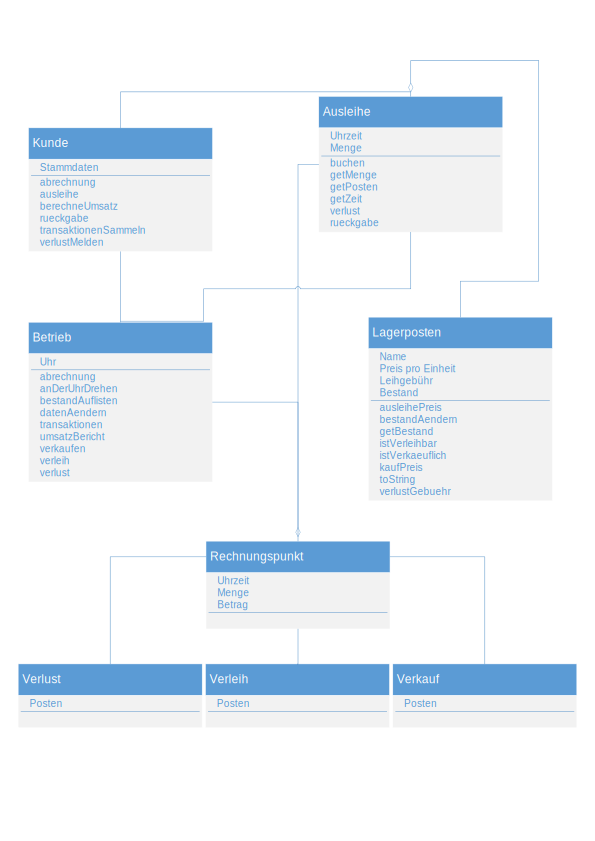
\includegraphics[width=\textwidth]{Klassendiagramm.pdf}
\newpage
\part{Methodenbeschreibung}
\section{Kunde}
\begin{description}
\item[\{set, get\}\{Name, VorName, ID, Straße, Hausnummer, PLZ, Ort\}]
Holt oder ändert die entsprechenden Werte.
\item[rueckgabe(posten, zeit, menge)]
Bucht eine gegebene Menge eines gegebenen Postens von den Ausleihen des Kunden zurück ins Lager
und stellt die Kosten der Ausleihe dem Kunden in Rechnung.\\
Exception wenn der Posten nicht ausgeliehen war oder die angegebene Menge die Leihmenge übersteigt.
\item[verlustMelden(posten, zeit, menge)]
Streicht eine gegebene Menge eines gegebenen Postens von den Ausleihen des Kunden\\
Exception wenn der Posten nicht ausgeliehen war oder die angegebene Menge die Leihmenge übersteigt.
und stellt dem Kunden die Verlustgebühr in Rechnung.
\item[ausleihe(ausleihe)]
Fügt eine Ausleihe dem Kundenkonto hinzu. Dabei wird diese gebucht.
\item[abrechnung(zeit) -> RechnungPosten{[]}]
Gibt alle ausstehenden Rechnungspunkte zurück und legt sie damit zu den bearbeiteten Rechnungspunkten.
\item[berechneUmsatz() -> geld]
Berechnet den gesamten Umsatz, der durch den Kunden verursacht wurde, d. h. der Wert aller bearbeiteten Rechnungspunkte.
\item[transaktionenSammeln() -> String{[]}]
Stellt alle Rechungspunkte und bestehenden Ausleihen zusammen.
\item[kaufen(posten, menge)]
Verkauft (entfernt Bestand) und stellt dem Kunden den Kaufpreis in Rechnung.
\end{description}
\section{Ausleihe}
\begin{description}
\item[buchen()]
Die Ausleihe tritt in Kraft: Entfernt die auszuleihende Menge des Posten aus dem Lager.
\item[getPosten() -> LagerPosten]
Gibt den Posten der geliehen wird, zurück.
\item[getMenge() -> menge]
Gibt die ausgeliehende / auszuleihende Menge zurück.
\item[getZeit() -> zeit]
Gibt die Startzeit der Ausleihe zurück.
\item[verlust(menge) -> menge]
Annuliert eine bestimmte Menge in der Ausleihe, gibt ggf. die Menge, die von anderen Ausleihen gedeckt wird, zurück.
\item[rueckgabe(menge) -> menge]
Bucht eine bestimmte Menge zurück, gibt ggf. die Menge, die von anderen Ausleihen gedeckt wird, zurück.
\end{description}
\section{LagerPosten}
\begin{description}
\item[toString() -> String]
gibt die Daten des Postens, zB in der Form \enquote{<Bestand> x <ID> <Name> (<Einheit>)} als String zurück
\item[istVerkaeuflich() -> boolean]
Bestimmt ob der Artikel verkäuflich ist.
\item[istVerleihbar() -> boolean]
Bestimmt ob der Artikel verleihbar ist.
\item[bestandAendern(menge)]
Ändert den Bestand um die angegebene Menge (positiv oder negativ). \\
Exception wenn Bestand negativ werden würde.
\item[getBestand() -> geld]
Gibt den aktuellen Lagerbestand zurück.
\item[ausleihePreis(zeit, menge) -> geld]
Bestimmt die Leihgebühr einer gegebenen Menge des Postens über eine gegebene Zeitspanne.
\item[kaufPreis(menge) -> geld]
Bestimmt den Kaufpreis einer gegebenen Menge des Postens.
\item[verlustGebuer(zeit, menge) -> geld]
Bestimmt die Gebühr, die bei Verlust einer gegebenen Menge des Postens nach gegebener Zeit entsteht.
\end{description}
\section{Betrieb}
\begin{description}
\item[main(args)]
Hauptmenü
\item[bestandAuflisten(modus)]
listet den Bestand, gefiltert nach Kriterien, die durch modus bestimmt werden (Gesamtbestand, verf. Verkaufsware, verf. Verleihware, oÄ), auf
\item[verkaufen()]
der Verkaufs-Menüpunkt
\item[verleih()]
der Verleih-Menüpunkt
\item[abrechnung(kundenID)]
rechnet alle ausstehenden Rechnungspunkte beim Kunden ab
\item[rückgabe()]
der Rückgabe-Menüpunkt
\item[verlust()]
der Verlust-Meldungs-Menüpunkt
\item[umsatzBericht()]
listet die Umsätze der Kunden auf
\item[datenAendern(kundenID)]
ändert die Daten eines Kunden (Menü)
\item[transaktionen(kundenID)]
zeigt die Transaktionen eines Kunden an
\item[anDerUhrDrehen(zeit)]
schreitet die Zeit voran
\end{description}
\part{Testfälle}
\begin{enumerate}
\item
Auflistung des Gesamtbestandes zum Kaufen und zum Verleihen.\\
\Rightarrow Liste mit n Elementen zum Verkaufen und n Elementen zum Verleihen
\item
Auflistung des Gesamtbestandes zum Kaufen und zum Verleihen nach einer Änderung um x.\\
\Rightarrow Liste mit n-x bzw. n+x Elementen zum Verkaufen und zum Verleihen
\item
Auflistung des aktuell verfügbaren Bestandes zum Ausleihen und zum Kaufen.
\Rightarrow Liste mit y Elemente unterschiedlich(nach Ausleihe oder Verkauf) bzw. gleich zur Liste des Gesamtbestandes. 
\item
Verleihen von verfügbaren, nicht verfügbaren (die größer sind als die verfügbaren Mengen) und nichtganzzahligen Mengen.
\Rightarrow Führt zu Veränderungen am Bestand der zurzeit verfügbaren Objekten 
\item
Verkauf von verfügbaren, nicht verfügbaren (die größer sind als die verfügbaren Mengen) und nichtganzzahligen Mengen.
\Rightarrow Führt zu Veränderungen am Gesammtbestand und am zurzeit verfügbaren Bestand
\item
Rückgabe von Mengen, die die Ausleihe übersteigen(sollte nicht möglich sein).
\item
Rückgabe testen:
-vollsändig
-unvollständig
-im teilweise oder vollständig beschädigten Zustand
\item
Abrechnung testen.
\item
Umsatzliste testen.
\item
Transaktionen auflisten.
\item
Kundendaten ändern .
\item
Neuen Kunden aufnehmen.
\item
Computer-Mensch Dialog überprüfen (auf Aktionen die möglich sind und welche die nicht möglich sind).
\item
Kauf von nicht verkäuflichen Objekten(sollte nicht möglich sein).
\item
Leih von von nicht verleihbaren Objekten(sollte nicht möglich sein).
\item
Zeitpunkt in die Vergangenheit ändern bzw. negative Zeitdauer(sollte nicht möglich sein).
\item
Zeitpunkt in die Zukunft ändern.

\end{enumerate}
\appendix
\newpage
\part{Eigenständigkeitserklärung}
Wir versichern hiermit, dass wir diese Arbeit selbständig verfasst, keine anderen Quellen und Hilfsmittel
als die angegebenen benutzt und die Stellen der Arbeit, die anderen Werken dem Wortlaut oder dem Sinn nach entnommen sind,
in jedem einzelnen Fall unter Angabe der Quelle als Entlehnung kenntlich gemacht haben.
Das gleiche gilt auch für eingefügte Zeichnungen, Kartenskizzen und Darstellungen.

\today, \includegraphics{UnterschriftJonaStubbe.png}

\today, 
\today,
\end{document}
